% Provenance (never printed): old terminale S material on the disappearance of
% mountain ranges (erosion, transport, sedimentation, isostatic rebound, the
% recycling of continental material). Owner (Sync 0/1): denudation rate,
% sediment load (bed, suspended, dissolved), isostatic rebound, detrital rock,
% diagenesis. Weathering, erosion, deposition are Book 1's (g5); hydrolysis and
% clay minerals g10.07's; discharge g10.08's; isostasy and Airy's model g11.03's;
% sedimentary basin g11.09's; mountain root g12.01's; metamorphism g12.03's;
% half-life is physics' (recalled in prose). Figures: figdata/grade-12/relief_decay.py
% (rates, decay curves, the Varden unconformity from figdata/shared/region.py).
\chapter{La destruction des montagnes}\label{ch:g12:destruction-of-mountains}

Vues depuis la Station spatiale internationale, les Appalaches, dans l'est
de l'Amérique du Nord, dessinent un motif frappant de longues crêtes
sombres et boisées et de vallées claires et cultivées, sur plus de
\qty{500}{km} dans la photographie ci-dessous. Les crêtes sont des couches
de roches dures qui ont été froissées en \omterm{def:g12:mountain-building:fold}{plis} serrés quand l'Afrique a
poussé contre l'Amérique du Nord, au Carbonifère et au Permien, il y a plus
de 250 millions d'années. Aujourd'hui, leur plus haut sommet, le mont
Mitchell, le point culminant de l'est du Mississippi, s'élève à
\qty{2037}{m} au-dessus du niveau de la mer, moins du quart de la hauteur
de l'Everest.
% ledger: photo:g12-appalachians, usgs:alleghanian, usgs:alleghanian-age, ics:base.Triassic, ncparks:mitchell (6684 ft), tht:everest (Book 1 row, 8848.86 m)

\begin{omfigure}
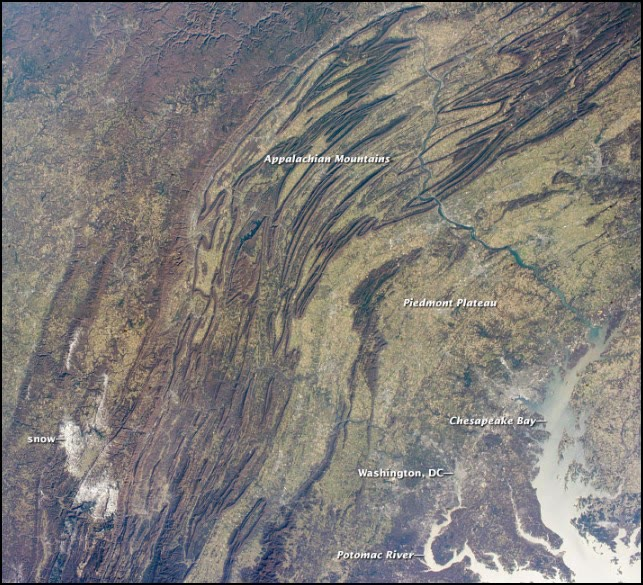
\includegraphics[width=0.6\linewidth]{images/book2/g12-iss-appalachians.jpg}

{\small Les Appalaches plissées, en crêtes et vallées, du nord-est de la
Pennsylvanie (en haut à droite) à la Virginie-Occidentale, photographiées
depuis la Station spatiale internationale le 17 novembre 2012. Les crêtes
boisées sont des couches de roches dures, les vallées cultivées des couches
plus tendres. Photographie NASA (domaine public).}
\end{omfigure}
% ledger: photo:g12-appalachians

Une chaîne de montagnes ne dure pas. Dès qu'elle s'élève, la pluie, la
glace et les rivières l'attaquent~; la roche qu'elles emportent finit dans
la mer, où elle devient une roche nouvelle. Ce chapitre mesure la vitesse
de ce processus, suit les débris jusqu'à l'endroit où ils redeviennent
pierre, et montre pourquoi une chaîne en cours d'usure continue de
s'élever pendant ce temps.

\begin{recall}
L'altération désagrège la roche sur place~; l'érosion emporte les débris,
et le dépôt les abandonne ailleurs (livre~1, année~5). L'\omterm{def:g10:soil-formation:chemical-weathering}{altération
chimique} transforme les feldspaths en \omterm{def:g10:soil-formation:clay}{minéraux argileux} par \omterm{def:g10:soil-formation:hydrolysis}{hydrolyse}
(\cref{ch:g10:soil-formation}). Le \omterm{def:g10:drainage-basins:discharge}{débit} d'une rivière est le volume d'eau
qui passe en un point en une seconde (\cref{ch:g10:drainage-basins}). La
croûte flotte sur le manteau en équilibre isostatique~; dans le modèle
d'Airy, une région dont la croûte est plus épaisse de $\Delta H$ se dresse
plus haut de $\Delta H\,(\rho_m - \rho_c)/\rho_m$
(\cref{ch:g11:lithosphere-asthenosphere}), et une haute chaîne repose sur
une \omterm{def:g12:continental-crust:root}{racine} de croûte épaisse (\cref{ch:g12:continental-crust}). Les
sédiments s'accumulent dans des \omterm{def:g11:fossil-fuel-geology:basin}{bassins sédimentaires}
(\cref{ch:g11:fossil-fuel-geology}). Les roches enfouies profondément dans
une chaîne de montagnes sont métamorphisées
(\cref{ch:g12:metamorphic-rocks}).
\end{recall}

\section{À quelle vitesse les terres s'usent-elles~?}

\begin{definition}[Taux de dénudation]\label{def:g12:destruction-of-mountains:denudation}
Le \emph{taux de dénudation}\index{taux de denudation@taux de dénudation}
d'une région est l'épaisseur moyenne de roche que l'altération et l'érosion
réunies lui enlèvent par unité de temps. On l'exprime en général en mètres
par million d'années (\unit{m/Ma}), ce qui revient à des millimètres par
millier d'années.
\end{definition}
% ledger: pb11:rates (rates in m/Myr), earle:loads

Comment mesurer quelque chose d'aussi lent~? Les rayons cosmiques qui
frappent le sol fabriquent un isotope rare, le béryllium~10, dans le quartz
des premiers mètres de roche. Plus une surface s'use lentement, plus chaque
grain reste longtemps près de la surface, et plus il accumule de
béryllium~10. Le mesurer dans le sable d'une rivière donne le \omterm{def:g12:destruction-of-mountains:denudation}{taux de
dénudation} moyen de tout le bassin situé en amont, sur les derniers
milliers à millions d'années.
% ledger: pb11:rates (10Be produced within a few metres of the surface; concentration reflects near-surface residence time; 10^3 to 10^6 years)

Une compilation de 1599 mesures de ce type a montré que les affleurements
de roche nue s'usent lentement, de \qty{12}{m/Ma} en moyenne (médiane
\qty{5.4}{m/Ma}), et jamais plus vite que \qty{140}{m/Ma}. Les \omterm{def:g10:drainage-basins:drainage-basin}{bassins
versants} entiers perdent bien plus, \qty{218}{m/Ma} en moyenne, mais avec
une médiane de seulement \qty{54}{m/Ma}~: quelques bassins rapides tirent
la moyenne vers le haut. Les plus rapides sont les plus pentus~: la pente
moyenne d'un bassin est le facteur qui prédit le mieux son taux. Les
bassins des régions sismiquement actives, où des montagnes s'élèvent,
s'érodent environ deux fois plus vite que ceux des régions calmes.
% ledger: pb11:rates

\begin{omfigure}
\begin{tikzpicture}
\begin{axis}[omrecord, xbar, xmode=log, log origin=infty, bar width=7pt, bar shift=0pt,
  width=0.62\linewidth, height=6.6cm, scale only axis, xmin=3, xmax=1000,
  ymin=0.4, ymax=10.6, ytick={1,...,10}, y tick label style={font=\scriptsize, align=right},
  yticklabels={{affleurements, médiane}, {affleurements, moyenne}, {fleuves du monde (bilan)}, {bassins, médiane},
    {Mississippi, avant 1900 (bilan)}, {bassins arides, moyenne}, {bassins calmes, moyenne}, {bassins, moyenne},
    {bassins sismiquement actifs, moyenne}, {bassins polaires, moyenne}},
  xlabel={taux de dénudation (\unit{m/Ma}), échelle logarithmique}, ymajorgrids=false,
  unbounded coords=discard, nodes near coords, nodes near coords align={horizontal}, nodes near coords style={font=\scriptsize},
  point meta=rawx, every node near coord/.append style={/pgf/number format/.cd, fixed, precision=0}]
% computed in figdata/grade-12/relief_decay.py; ledger: pb11:rates, mm10:mississippi, kammerer:mississippi, earle:loads, cm95:crust
\addplot[fill=omThm!45, draw=omThm, every node near coord/.append style={/pgf/number format/.cd, fixed, precision=1}] table[x=measured, y=idx] {figdata/out/grade-12-relief_decay-rates.dat};
\addplot[fill=omDef!45, draw=omDef] table[x=budget, y=idx] {figdata/out/grade-12-relief_decay-rates.dat};
\end{axis}
\end{tikzpicture}

{\small \omterm{def:g12:destruction-of-mountains:denudation}{Taux de dénudation} mesurés avec le béryllium~10 (en rouge~: 1599
mesures, dont 1149 dans du sable de rivière) et deux taux calculés dans ce
chapitre à partir des sédiments que transportent les fleuves (en bleu).
Sources~: Portenga et Bierman (2011)~; Meade et Moody (2010)~; Syvitski et
ses collègues (2005).}
\end{omfigure}
% values: world_m_per_myr 43.5, miss_before_1900_m_per_myr 55.8 (relief_decay.py)

\section{Les rivières emportent les montagnes}

Une grande partie de ce qui est arraché aux terres les quitte par les
rivières.

\begin{definition}[Charge sédimentaire]\label{def:g12:destruction-of-mountains:load}
La \emph{charge sédimentaire}\index{charge sedimentaire@charge sédimentaire}
d'une rivière est la matière qu'elle transporte, sous trois formes~: la
\emph{charge de fond}\index{charge de fond}, de gros grains roulés, poussés
ou sautant sur le fond~; la \emph{charge en suspension}\index{charge en suspension},
de petits grains maintenus dans l'eau en mouvement~; et la \emph{charge
dissoute}\index{charge dissoute}, des ions en solution, comme le calcium
et le chlorure, laissés par l'\omterm{def:g10:soil-formation:chemical-weathering}{altération chimique}.
\end{definition}
% ledger: earle:loads

En moyenne, la \omterm{def:g12:destruction-of-mountains:load}{charge dissoute} représente environ \qty{15}{\percent} de la
masse transportée par une rivière. Plus l'eau est rapide, plus les grains
qu'elle peut soulever sont gros. Un grain de sable de \qty{1}{mm} est
arraché au fond à environ \qty{20}{cm/s}, et une fois en mouvement il reste
en suspension jusqu'à ce que le courant tombe sous \qty{10}{cm/s}. Les
grains de silt sont plus difficiles à soulever que le sable, parce qu'ils
collent entre eux~: un grain de \qty{0.01}{mm} demande \qty{60}{cm/s} pour
être arraché, mais un courant de \qty{0.1}{cm/s} le maintient ensuite en
suspension. C'est pourquoi les rivières en crue sont brunes, et pourquoi la
boue la plus fine voyage jusqu'à la mer.
% ledger: earle:loads

\begin{omfigure}
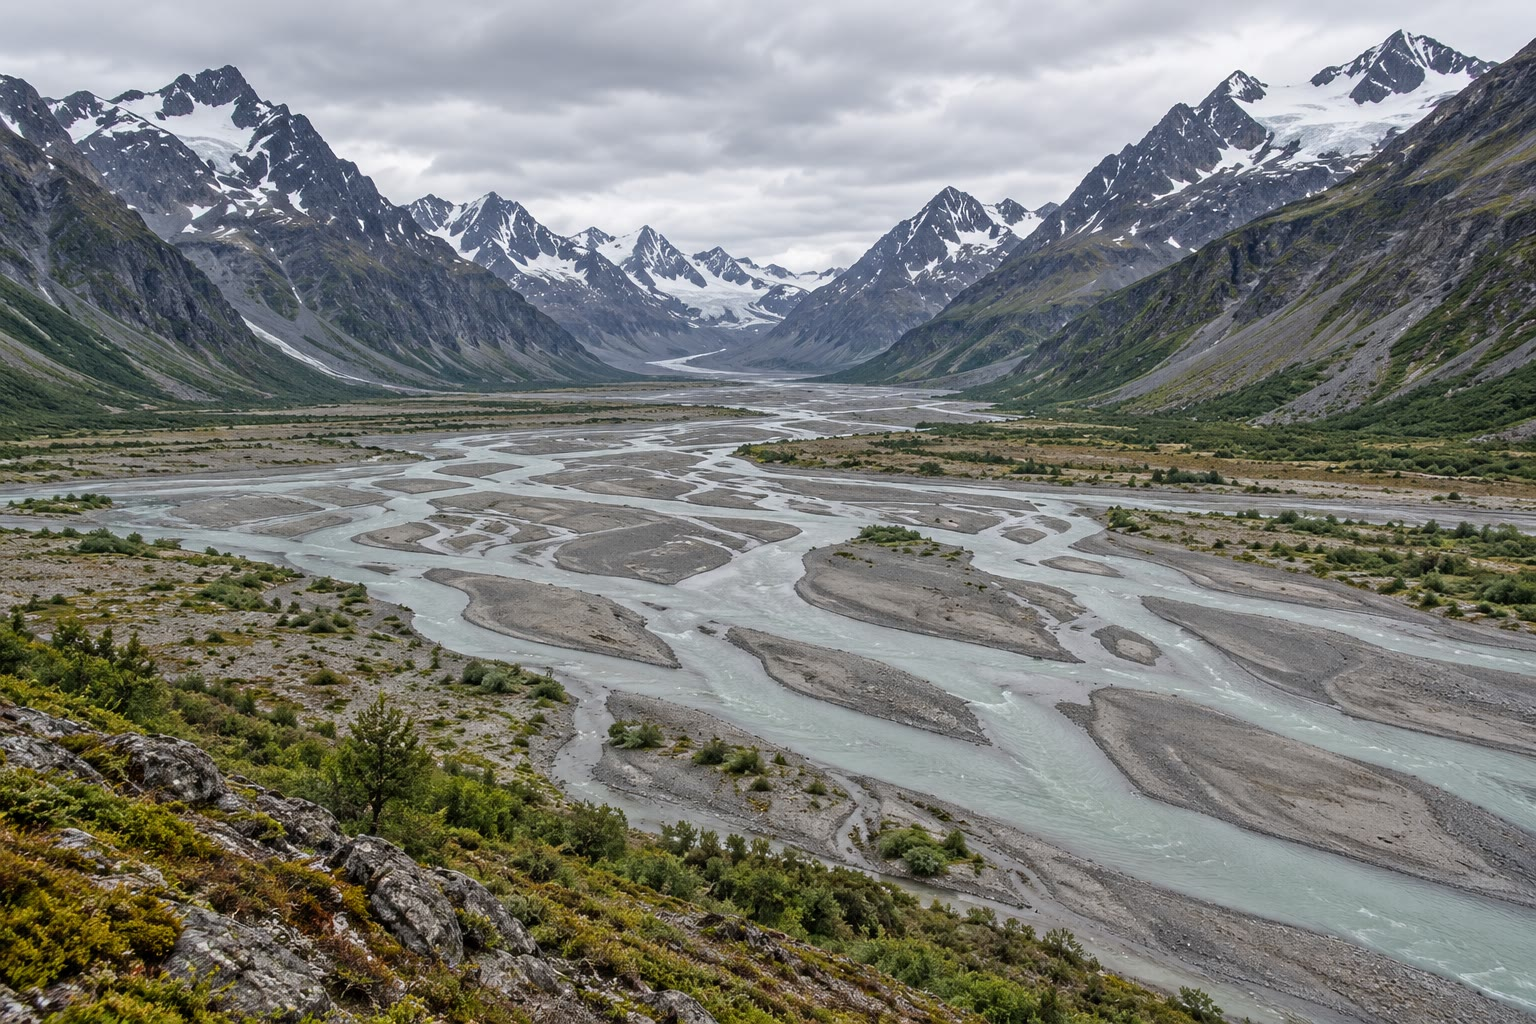
\includegraphics[width=0.66\linewidth]{images/book2/ai/g12-braided-river.jpg}

{\small Une rivière en tresses dans une vallée glaciaire de montagne~: des
chenaux peu profonds se séparent et se rejoignent entre des bancs de
graviers que l'eau ne déplace qu'en crue. Illustration générée par IA.}
\end{omfigure}

Mesurer ce que transporte une rivière donne une seconde façon de trouver un
\omterm{def:g12:destruction-of-mountains:denudation}{taux de dénudation}.

\begin{method}[Un bilan d'érosion]\label{met:g12:destruction-of-mountains:budget}
\begin{enumerate}
  \item Prendre la masse de sédiments que la rivière transporte en un an,
        et y ajouter la \omterm{def:g12:destruction-of-mountains:load}{charge dissoute} (si seule la charge solide est
        connue, la diviser par $0.85$).
  \item Diviser par la masse volumique de la roche, environ
        \qty{2830}{kg/m^3} pour la \omterm{def:g12:continental-crust:continental-crust}{croûte continentale}, pour obtenir le
        volume de roche enlevé chaque année.
  \item Diviser par la surface du \omterm{def:g10:drainage-basins:drainage-basin}{bassin versant}~: c'est l'épaisseur
        enlevée chaque année.
  \item Multiplier par $10^6$ pour l'exprimer en mètres par million
        d'années.
\end{enumerate}
\end{method}
% ledger: earle:loads, cm95:crust

\begin{example}[Le Mississippi]\label{ex:g12:destruction-of-mountains:mississippi}
Avant 1900, le système Missouri--Mississippi transportait chaque année
environ 400 millions de tonnes de sédiments jusqu'à la mer, depuis un
bassin d'environ \qty{2980000}{km^2}. Avec la \omterm{def:g12:destruction-of-mountains:load}{charge dissoute},
$400/0.85 \approx 471$ millions de tonnes, soit
$\num{4.71e11}/2830 \approx \qty{1.66e8}{m^3}$ de roche par an. Étalé sur
$\qty{2.98e12}{m^2}$, cela fait une couche
\[
  \frac{\num{1.66e8}}{\num{2.98e12}} \approx \qty{5.6e-5}{m}
  \text{ par an, soit environ } \qty{56}{m/Ma}.
\]
Entre 1987 et 2006, le fleuve n'a plus transporté que 145 millions de
tonnes par an, ce qui donne environ \qty{20}{m/Ma}~: les barrages
construits sur le Missouri dans les années 1950 retiennent environ 100 à
150 millions de tonnes par an, et d'autres ouvrages en retiennent davantage.
\end{example}
% ledger: mm10:mississippi, kammerer:mississippi, earle:loads, cm95:crust
% values: miss_before_1900_m_per_myr 55.8, miss_1987_2006_m_per_myr 20.2 (relief_decay.py)

On peut faire le même bilan pour le monde entier. Avant que l'homme ne
modifie les fleuves, ceux-ci apportaient aux côtes environ 15.5~milliards
de tonnes de sédiments solides par an~; avec la \omterm{def:g12:destruction-of-mountains:load}{charge dissoute}, cela fait
environ \qty{6.4}{km^3} de roche par an, pris aux \qty{1.48e8}{km^2} des
continents~: un \omterm{def:g12:destruction-of-mountains:denudation}{taux de dénudation} moyen d'environ \qty{43}{m/Ma}, proche
de la médiane des mesures au béryllium~10. Les hommes ont depuis modifié
les deux termes~: l'érosion des sols a augmenté d'environ 2.3~milliards de
tonnes par an ce que les fleuves emportent, mais plus de 100~milliards de
tonnes de sédiments sont aujourd'hui retenues derrière des barrages.
% ledger: syvitski:modern-flux (Book 1 row, prehuman 15.5 Gt/yr with bed load), sy05:humans, data:etopo1 (land fraction 0.290, grade-11 hypsometry), cm95:crust
% values: world_volume_km3_per_yr 6.44, land_area_km2 1.48e8, world_m_per_myr 43.5 (relief_decay.py)

\section{Du sédiment à la roche}

Ce que transportent les rivières se dépose là où le courant ralentit~: dans
les vallées et les lacs, sur les deltas, et surtout dans les \omterm{def:g11:fossil-fuel-geology:basin}{bassins
sédimentaires} des marges continentales. Couche après couche, le sédiment est
enfoui, et il se transforme lentement en roche.

\begin{definition}[Roche détritique~; diagenèse]\label{def:g12:destruction-of-mountains:diagenesis}
Une \emph{roche détritique}\index{roche detritique@roche détritique} (ou
roche clastique) est une roche sédimentaire faite de fragments, les clastes,
de roches et de minéraux plus anciens. La
\emph{diagenèse}\index{diagenese@diagenèse} est l'ensemble des
transformations qui changent un sédiment enfoui en roche à basse
température~: la \emph{compaction}, quand le poids des couches situées
au-dessus chasse l'eau et l'air, puis la \emph{cimentation}, quand des
minéraux qui cristallisent à partir de l'eau des pores (calcite, quartz,
hématite, \omterm{def:g10:soil-formation:clay}{minéraux argileux}) collent les grains entre eux.
\end{definition}
% ledger: earle:clastic

On nomme les \omterm{def:g12:destruction-of-mountains:diagenesis}{roches détritiques} d'après la taille de leurs clastes~:
\begin{itemize}
  \item un \textbf{conglomérat} est fait de clastes arrondis de plus de
        \qty{2}{mm}, une \textbf{brèche} de clastes anguleux~;
  \item un \textbf{grès} est fait de sable, des grains compris entre
        \qty{2}{mm} et \qty{0.063}{mm}, le plus souvent de quartz, le
        minéral qui résiste le mieux à l'altération~;
  \item une \textbf{lutite} contient au moins \qty{75}{\percent} de silt et
        d'argile~; c'est une argilite feuilletée si elle se débite en
        couches minces.
\end{itemize}
% ledger: earle:clastic

\begin{omfigure}
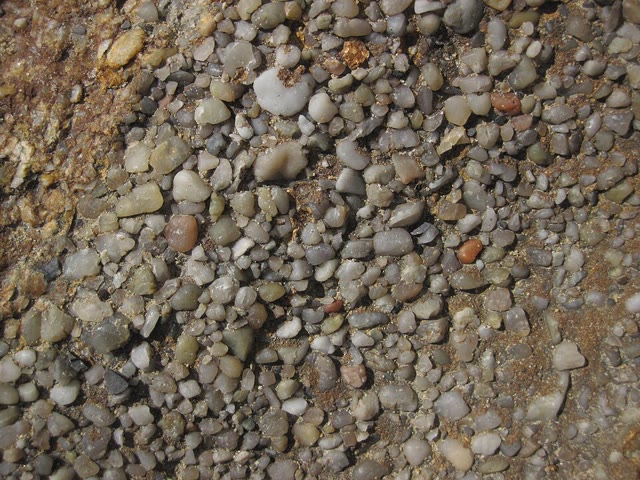
\includegraphics[width=0.5\linewidth]{images/book2/g12-stjohn-conglomerate.jpg}

{\small Un conglomérat à galets de quartz de l'Ohio, d'âge carbonifère~:
des galets arrondis de quartz, cimentés par un sable plus fin. Photographie
James St.~John (CC~BY~2.0).}
\end{omfigure}
% ledger: photo:g12-conglomerate, ics:base.Carboniferous, ics:base.Permian (Lower Pennsylvanian lies in the Carboniferous)

Les clastes enregistrent le voyage. Des galets arrondis ont longtemps roulé
dans une rivière ou sur une plage~; des fragments anguleux n'ont presque
pas voyagé. Un grès fait presque uniquement de quartz provient d'une roche
altérée pendant longtemps, jusqu'à ce que les autres minéraux se soient
changés en argile.
% ledger: earle:clastic (rounded/angular, most sand grains quartz, the most resistant mineral)

\section{La racine remonte}

Si l'érosion ne faisait qu'enlever de la roche au sommet d'une chaîne, une
chaîne haute de \qty{2}{km}, usée à \qty{200}{m/Ma}, disparaîtrait en dix
millions d'années. Mais la chaîne flotte sur le manteau. À mesure que de la
roche est enlevée au sommet, la colonne s'allège, et elle remonte.

\begin{definition}[Rebond isostatique]\label{def:g12:destruction-of-mountains:rebound}
Le \emph{rebond isostatique}\index{rebond isostatique} est la remontée
d'une région de la \omterm{def:g11:lithosphere-asthenosphere:lithosphere}{lithosphère} quand une charge lui est retirée --- roche
usée par l'érosion, ou calotte glaciaire qui fond --- jusqu'au
rétablissement de l'\omterm{def:g11:lithosphere-asthenosphere:isostasy}{isostasie}.
\end{definition}
% ledger: sella07:gia (rebound after ice unloading)

\begin{proposition}[Érosion et rebond]\label{prop:g12:destruction-of-mountains:rebound}
Dans le modèle d'Airy, quand l'érosion enlève une épaisseur $e$ de croûte
de masse volumique $\rho_c$ à une région en équilibre isostatique sur un
manteau de masse volumique $\rho_m$, la surface ne s'abaisse que de
\[
  \Delta h = e\left(1 - \frac{\rho_c}{\rho_m}\right),
\]
tandis que la base de la croûte remonte de $e\,\rho_c/\rho_m$.
\end{proposition}

\begin{proof}
Enlever $e$ au sommet amincit la croûte de $e$. D'après le modèle d'Airy,
une croûte plus mince de $e$ se trouve plus bas de $e\,(\rho_m - \rho_c)/\rho_m = e(1 -
\rho_c/\rho_m)$. Le sommet de la croûte s'est abaissé de cette quantité, et
son épaisseur a diminué de $e$~: sa base est donc remontée de $e - e(1 -
\rho_c/\rho_m) = e\,\rho_c/\rho_m$.
\end{proof}

Avec $\rho_c = \qty{2830}{kg/m^3}$ et $\rho_m = \qty{3380}{kg/m^3}$, $1 -
\rho_c/\rho_m \approx 0.163$. Enlever \qty{1}{km} de roche n'abaisse la
surface que d'environ \qty{163}{m}~: les \qty{837}{m} restants sont
compensés par la remontée de toute la colonne. Pour abaisser une chaîne de
\qty{2000}{m}, l'érosion doit enlever environ
$2000/0.163 \approx \qty{12300}{m}$ de roche. Des roches qui se trouvaient
à plus de \qty{12}{km} de profondeur, roches métamorphiques et granites
formés dans les profondeurs de la chaîne, arrivent en surface~: c'est
pourquoi les vieilles chaînes usées montrent des schistes, des gneiss et
des granites sur de vastes étendues.
% ledger: cm95:crust, data:prem (rho 3.38 below the Moho)
% values: rebound_fraction 0.16272, lowering_per_km_m 162.7, root_rise_per_km_m 837.3, eroded_for_2000m_km 12.29 (relief_decay.py)

\begin{omfigure}
\begin{tikzpicture}[x=1cm, y=1cm, font=\scriptsize]
  % three columns: before, after erosion without rebound, after rebound
  \foreach \i/\top/\base/\lab in {0/3.0/-3.2/{une chaîne en équilibre isostatique}, 1/2.0/-3.2/{l'érosion enlève $e$}, 2/2.84/-2.36/{la colonne remonte}} {
    \begin{scope}[xshift=\i*4.6cm]
      \fill[omLithPeridotite!45] (0,-3.6) rectangle (3.4,-0.6);
      \fill[omLithGranite!55, draw=black!60] (0.5,\base) -- (0.5,0) -- (1.0,\top) -- (2.4,\top) -- (2.9,0) -- (2.9,\base) -- cycle;
      \fill[omLithGranite!55, draw=black!60] (0,0) rectangle (0.5,-0.6);
      \fill[omLithGranite!55, draw=black!60] (2.9,0) rectangle (3.4,-0.6);
      \draw[black!40, densely dashed] (-0.1,0) -- (3.5,0);
      \node[anchor=north, align=center, text width=3.4cm] at (1.7,-3.75) {\lab};
    \end{scope}
  }
  % eroded slab, middle panel
  \draw[omThm, densely dashed] (4.6+1.0,3.0) -- (4.6+2.4,3.0);
  \draw[omThm, |-|] (4.6+2.65,3.0) -- node[right] {$e$} (4.6+2.65,2.0);
  % right panel: the old top and base
  \draw[omThm, densely dashed] (9.2+1.0,3.0) -- (9.2+2.4,3.0);
  \draw[omThm, densely dashed] (9.2+0.5,-3.2) -- (9.2+2.9,-3.2);
  \draw[-{Stealth}, omDef, line width=0.9pt] (9.2+1.7,-3.15) -- (9.2+1.7,-2.45);
  \node[omDef, anchor=west] at (9.2+3.0,-2.8) {la racine remonte};
  \node[anchor=west] at (9.2+3.0,2.95) {surface abaissée};
  \node[anchor=west] at (9.2+3.0,2.55) {de $0.16\,e$ seulement};
  \draw[black!60, |-|] (9.2+2.65,3.0) -- (9.2+2.65,2.84);
  % labels
  \node[anchor=west] at (3.45,-2.1) {manteau};
  \node at (1.7,-1.5) {croûte};
\end{tikzpicture}

{\small Érosion et \omterm{def:g12:destruction-of-mountains:rebound}{rebond isostatique} (schéma, hauteurs sans échelle). À
gauche~: une chaîne en équilibre isostatique, avec sa \omterm{def:g12:continental-crust:root}{racine}. Au centre~:
l'érosion enlève une épaisseur $e$ au sommet. À droite~: la colonne allégée
remonte jusqu'au rétablissement de l'\omterm{def:g11:lithosphere-asthenosphere:isostasy}{isostasie}~; la surface ne finit que
$0.163\,e$ plus bas qu'au départ, et la \omterm{def:g12:continental-crust:root}{racine} est remontée de
$0.837\,e$.}
\end{omfigure}

On peut observer aujourd'hui ce même rebond là où une charge a disparu
rapidement. La calotte glaciaire qui couvrait une grande partie du Canada au
dernier maximum glaciaire était la plus épaisse autour de la baie
d'Hudson. Cette glace a fondu, et le sol y remonte encore~: d'environ
\qty{10}{mm} par an, d'après les mesures GPS, soit \qty{10000}{m/Ma},
environ cinquante fois le \omterm{def:g12:destruction-of-mountains:denudation}{taux de dénudation} moyen des \omterm{def:g10:drainage-basins:drainage-basin}{bassins versants}.
Plus au sud, au-delà des Grands Lacs, le sol s'enfonce de 1 à \qty{2}{mm}
par an.
% ledger: sella07:gia, pb11:rates

\section{Combien de temps dure une chaîne~?}

Plus un bassin est pentu, plus il s'érode vite~; pour les grands bassins, on
a trouvé le \omterm{def:g12:destruction-of-mountains:denudation}{taux de dénudation} proportionnel à leur relief moyen. Prenons le
modèle le plus simple qui traduise cette relation.

\begin{proposition}[La décroissance exponentielle d'une chaîne]\label{prop:g12:destruction-of-mountains:decay}
Soit $h(t)$ l'altitude moyenne d'une chaîne au-dessus des plaines qui
l'entourent. Si le \omterm{def:g12:destruction-of-mountains:denudation}{taux de dénudation} vaut $E = k\,h$, avec $k$ une
constante, et si l'\omterm{def:g11:lithosphere-asthenosphere:isostasy}{isostasie} est rétablie en permanence, alors
\[
  h(t) = h_0\, e^{-f k t}, \qquad f = 1 - \frac{\rho_c}{\rho_m},
\]
où $h_0$ est l'altitude à $t = 0$. L'altitude est divisée par $e$ tous les
$\tau = 1/(fk)$, et par deux tous les $\tau \ln 2$.
\end{proposition}

\begin{proof}
En un temps court $\mathrm{d}t$, l'érosion enlève une épaisseur $E\,\mathrm{d}t
= k h\,\mathrm{d}t$, et d'après la proposition précédente la surface
s'abaisse de $f k h\,\mathrm{d}t$. Donc $h' = -fk\,h$, et les solutions de
cette équation sont $h(t) = h_0\,e^{-fkt}$. À $t = \tau$, $h = h_0/e$~;
$h = h_0/2$ quand $fkt = \ln 2$.
\end{proof}

Les mesures sur les grands bassins donnent $k$~: sans aucun soulèvement,
leur relief tomberait au dixième en 11 millions d'années environ. Donc
$e^{-11k} = 0.1$, et $k =
\ln 10/11 \approx 0.209$ par million d'années. Sans rebond ($f = 1$), la
constante de temps serait $1/k \approx 4.8$ millions d'années. Avec le
rebond, $f
\approx 0.163$ et
\[
  \tau = \frac{1}{0.163 \times 0.209} \approx 29 \text{ millions d'années},
\]
et l'altitude moyenne est divisée par deux tous les
$29 \ln 2 \approx 20$ millions d'années~: le rebond fait durer une chaîne
environ six fois plus longtemps.
% ledger: ahnert70:decay, cm95:crust, data:prem
% values: k_per_myr 0.20933, tau_none_myr 4.777, tau_rebound_myr 29.36, half_rebound_myr 20.35, half_none_myr 3.31 (relief_decay.py)

\begin{omfigure}
\begin{tikzpicture}
\begin{axis}[omrecord, width=0.7\linewidth, height=5.4cm, xmin=0, xmax=100, ymin=0, ymax=2100,
  xlabel={temps (millions d'années)}, ylabel={altitude moyenne (\unit{m})},
  xtick={0,20,...,100}, ytick={0,500,...,2000}]
% computed in figdata/grade-12/relief_decay.py; ledger: ahnert70:decay, cm95:crust, data:prem
\addplot[omProp, line width=1.1pt, densely dashed] table[x=t_Myr, y=h_none] {figdata/out/grade-12-relief_decay-curve.dat};
\addplot[omDef, line width=1.1pt] table[x=t_Myr, y=h_rebound] {figdata/out/grade-12-relief_decay-curve.dat};
\draw[black!45, densely dotted] (axis cs:20.35,0) -- (axis cs:20.35,1000) -- (axis cs:0,1000);
\draw[omProp, line width=0.4pt] (axis cs:9,304) -- (axis cs:33,215);
\coordinate (none) at (axis cs:33.5,215);
\coordinate (reb) at (axis cs:45,780);
\end{axis}
\node[font=\scriptsize, text=omProp, anchor=west] at (none) {sans rebond};
\node[font=\scriptsize, text=omDef, anchor=south west] at (reb) {avec rebond};
\end{tikzpicture}

{\small L'altitude moyenne d'une chaîne haute de \qty{2000}{m}, usée à un
rythme proportionnel à sa hauteur, avec et sans \omterm{def:g12:destruction-of-mountains:rebound}{rebond isostatique}~; avec
rebond, il reste la moitié de l'altitude au bout de 20 millions d'années
(en pointillés). Constante de vitesse d'après Ahnert (1970)~; masses
volumiques de la croûte et du manteau situé sous le \omterm{def:g11:seismic-structure:moho}{Moho}.}
\end{omfigure}

Les Appalaches mettent ce tableau à l'épreuve. Leur collision s'est achevée
au Permien, il y a plus de 250 millions d'années. C'est plus de douze fois
le temps que met le modèle à diviser l'altitude par deux~: $2000 \times e^{-250/29} \approx
\qty{0.4}{m}$. Pourtant, le mont Mitchell s'élève encore à \qty{2037}{m}
au-dessus de la mer. Le modèle seul ne peut pas expliquer le relief
actuel~: la région a dû être soulevée de nouveau depuis, ou s'éroder plus
lentement que le modèle ne le suppose.
% ledger: usgs:alleghanian, usgs:alleghanian-age, ics:base.Triassic, ncparks:mitchell, ahnert70:decay
% values: h_after_250myr_rebound_m 0.40 (relief_decay.py)

Les montagnes sont donc recyclées. La roche usée d'une chaîne finit dans
des \omterm{def:g11:fossil-fuel-geology:basin}{bassins sédimentaires}, où elle devient \omterm{def:g12:destruction-of-mountains:diagenesis}{roche détritique}~; une partie
de cette roche est enfouie assez profondément pour être métamorphisée ou
même pour fondre, une partie est entraînée dans le manteau à une \omterm{def:g11:subduction-zones:subduction}{zone de
subduction} (\cref{ch:g12:subduction-magmatism}), et une partie est de
nouveau plissée en une nouvelle chaîne quand deux continents entrent en
collision.
% ledger: ss09:balance (sediment subducted), earle:collision (sediments of both margins in the mountains)

\begin{omfigure}
\begin{tikzpicture}
\begin{axis}[omsection, x=1.25cm, y=0.003125cm, xmin=0, xmax=9.49, ymin=-700, ymax=650,
  xlabel={distance à A (\unit{km})}, ylabel={altitude (\unit{m})},
  ytick={-600,-300,0,300,600}, tick label style={font=\scriptsize}, unbounded coords=jump]
% shared region tables (figdata/shared/region.py); unconformity from figdata/grade-12/relief_decay.py; ledger: region:name
\addplot[fill=black!8, draw=black!50, line width=0.3pt, even odd rule] table {figdata/out/shared-region-section-unit-schist.dat};
\addplot[fill=icsTriassic!20, draw=black!50, line width=0.3pt, even odd rule] table {figdata/out/shared-region-section-unit-sandstone.dat};
\addplot[fill=icsJurassic!25, draw=black!50, line width=0.3pt, even odd rule] table {figdata/out/shared-region-section-unit-limestone.dat};
\addplot[fill=icsJurassic!8, draw=black!50, line width=0.3pt, even odd rule] table {figdata/out/shared-region-section-unit-shale.dat};
\addplot[fill=icsCretaceous!20, draw=black!50, line width=0.3pt, even odd rule] table {figdata/out/shared-region-section-unit-chalk.dat};
\addplot[fill=omLithAlluv, draw=black!50, line width=0.3pt, even odd rule] table {figdata/out/shared-region-section-unit-alluvium.dat};
\addplot[black, line width=0.7pt] table {figdata/out/shared-region-section-ground.dat};
\addplot[omThm, line width=1.4pt] table[x=s_km, y=z_m] {figdata/out/grade-12-relief_decay-unconformity.dat};
\addplot[fault] table {figdata/out/shared-region-section-fault.dat};
\node[anchor=south east, font=\small\bfseries] at (axis cs:0,650) {A};
\node[anchor=south west, font=\small\bfseries] at (axis cs:9.49,650) {B};
\node[font=\scriptsize, fill=white, inner sep=1pt] at (axis cs:1.2,-520) {schiste, environ 480 Ma};
\coordinate (unc) at (axis cs:1.6,-300);
\end{axis}
\node[font=\scriptsize, text=omThm, anchor=west, fill=white, inner sep=1pt] at ([xshift=4pt]unc) {la discordance};
\end{tikzpicture}

\smallskip
{\small\tikz\fill[black!8, draw=black!50] (0,0) rectangle (0.35,0.22);~schiste \quad
\tikz\fill[icsTriassic!20, draw=black!50] (0,0) rectangle (0.35,0.22);~grès (Trias) \quad
\tikz\fill[icsJurassic!25, draw=black!50] (0,0) rectangle (0.35,0.22);~calcaire \quad
\tikz\fill[icsJurassic!8, draw=black!50] (0,0) rectangle (0.35,0.22);~argilite \quad
\tikz\fill[icsCretaceous!20, draw=black!50] (0,0) rectangle (0.35,0.22);~craie \quad
\omve{2.5}}

{\small Coupe A--B à travers les collines de Varden, avec la discordance en
rouge~: la base plane sur laquelle le grès du Trias s'est déposé en
travers du socle de schiste, plissée et faillée par la suite. Données~: le
modèle de la région propre à la série.}
\end{omfigure}
% values: unconformity sampled from region.contact_elevation('sandstone'); varden_gap_myr 58.1 (relief_decay.py)

Les collines de Varden gardent la trace d'un tel cycle. Leur socle est un
schiste, métamorphisé il y a environ 480 millions d'années, dans lequel un
granite s'est mis en place il y a environ 310 millions d'années --- tous
deux formés à des kilomètres sous la surface d'une ancienne chaîne de
montagnes. Pourtant, le grès du Trias, déposé à partir d'il y a environ
252 millions d'années, repose directement sur eux, sur une surface plane~:
la discordance. En moins de 60 millions d'années, cette ancienne chaîne a
été usée jusqu'à n'être plus qu'une plaine, et ses roches profondes ont été
amenées en surface. La mer s'est ensuite étendue sur la plaine et l'a
recouverte.
% ledger: region:name (model: schist 480 Ma, granite 310 Ma, erosion, unconformity, Triassic cover), ics:base.Triassic
% values: varden_gap_myr 58.1 (relief_decay.py)

\section{Exercices}

\begin{exercise}[$\star$]\label{exo:g12:destruction-of-mountains:1}
Donner le mot~: (a) l'épaisseur moyenne de roche enlevée à une région par
unité de temps~; (b) les grains qu'une rivière roule et fait sauter sur son
lit~; (c) les ions qu'une rivière transporte en solution~; (d) les
transformations qui changent un sédiment enfoui en roche~; (e) la remontée
de la \omterm{def:g11:lithosphere-asthenosphere:lithosphere}{lithosphère} quand une charge lui est retirée.
\end{exercise}

\begin{exercise}[$\star$]\label{exo:g12:destruction-of-mountains:2}
Nommer la \omterm{def:g12:destruction-of-mountains:diagenesis}{roche détritique}~: (1) des galets arrondis de
\qtyrange{5}{20}{mm} cimentés entre eux~; (2) des grains de quartz de
\qty{0.3}{mm}~; (3) une roche faite à \qty{90}{\percent} de silt et
d'argile, qui se débite en feuillets minces~; (4) des fragments anguleux de
\qty{3}{cm}.
\end{exercise}

\begin{exercise}[$\star$]\label{exo:g12:destruction-of-mountains:3}
Convertir en millimètres par an~: (1) \qty{54}{m/Ma}~; (2) \qty{218}{m/Ma}~;
(3) convertir le soulèvement de \qty{10}{mm} par an près de la baie
d'Hudson en \unit{m/Ma}.
\end{exercise}

\begin{exercise}[$\star$]\label{exo:g12:destruction-of-mountains:4}
Une rivière transporte 60 millions de tonnes de sédiments solides par an.
Estimer sa \omterm{def:g12:destruction-of-mountains:load}{charge dissoute}, sachant que la \omterm{def:g12:destruction-of-mountains:load}{charge dissoute} représente en
moyenne \qty{15}{\percent} de la masse totale transportée.
\end{exercise}

\begin{exercise}[$\star$]\label{exo:g12:destruction-of-mountains:5}
Ranger dans l'ordre, de la surface vers la profondeur, ce qui arrive à un
grain de quartz d'un granite~: le dépôt dans un bassin, l'altération du
granite, l'enfouissement sous des couches plus jeunes, le transport par une
rivière, la cimentation.
\end{exercise}

\begin{exercise}[$\star\star$]\label{exo:g12:destruction-of-mountains:6}
Un courant ralentit de \qty{30}{cm/s} à \qty{5}{cm/s}. À l'aide des
valeurs du chapitre, dire ce qui arrive, à chaque vitesse, à un grain de
sable de \qty{1}{mm} posé sur le fond et à un grain de silt de
\qty{0.01}{mm} déjà en suspension.
\end{exercise}

\begin{exercise}[$\star\star$]\label{exo:g12:destruction-of-mountains:7}
Un bassin de \qty{50000}{km^2} envoie chaque année 4 millions de tonnes de
sédiments solides à la mer. Établir son bilan d'érosion, \omterm{def:g12:destruction-of-mountains:load}{charge dissoute}
comprise, avec $\rho =
\qty{2830}{kg/m^3}$. Comparer à la médiane des taux mesurés au béryllium~10
dans les bassins.
\end{exercise}

\begin{exercise}[$\star\star$]\label{exo:g12:destruction-of-mountains:8}
(1) Calculer $1 - \rho_c/\rho_m$ pour $\rho_c = \qty{2700}{kg/m^3}$ et
$\rho_m = \qty{3300}{kg/m^3}$. (2) De combien la surface s'abaisse-t-elle
quand \qty{1}{km} de roche est érodé~? (3) Comparer à la valeur du
chapitre.
\end{exercise}

\begin{exercise}[$\star\star$]\label{exo:g12:destruction-of-mountains:9}
Un granite a cristallisé à environ \qty{8}{km} de profondeur sous une
chaîne. (1) Quelle épaisseur de roche l'érosion doit-elle enlever pour
l'amener en surface~? (2) De combien la surface moyenne s'abaisse-t-elle
pendant ce temps~? (3) À \qty{200}{m/Ma}, combien de temps cela prend-il~?
\end{exercise}

\begin{exercise}[$\star\star$]\label{exo:g12:destruction-of-mountains:10}
L'altitude moyenne des continents est d'environ \qty{794}{m}. (1) À
\qty{43}{m/Ma}, combien de temps l'érosion mettrait-elle à enlever une
couche de cette épaisseur~? (2) Combien de temps, si l'on tient compte du
\omterm{def:g12:destruction-of-mountains:rebound}{rebond isostatique} et que le taux reste le même~? (3) Pourquoi les
continents se dressent-ils pourtant encore au-dessus de la mer au bout de
4~milliards d'années~?
\end{exercise}

\begin{exercise}[$\star\star$]\label{exo:g12:destruction-of-mountains:11}
Plus de 100~milliards de tonnes de sédiments sont retenues derrière des
barrages construits pour la plupart au cours des cinquante dernières
années. (1) Quel volume de roche cela représente-t-il, à
\qty{2830}{kg/m^3}~? (2) Combien d'années de la charge solide mondiale
d'avant l'homme, 15.5~milliards de tonnes par an, cela représente-t-il~?
\end{exercise}

\begin{exercise}[$\star\star\star$]\label{exo:g12:destruction-of-mountains:12}
Montrer que, dans le modèle du chapitre, le \omterm{def:g12:destruction-of-mountains:denudation}{taux de dénudation} d'une chaîne
vaut $E(t) = k h_0 e^{-fkt}$. Calculer l'épaisseur totale de roche enlevée
pendant que l'altitude moyenne tombe de $h_0$ à 0, et expliquer le résultat
à l'aide de la proposition sur le rebond.
\end{exercise}

\begin{exercise}[$\star\star\star$]\label{exo:g12:destruction-of-mountains:13}
Près de la baie d'Hudson, le sol remonte de \qty{10}{mm} par an. (1) Si ce
rythme restait le même, de combien remonterait-il en 1000 ans~? (2) La
remontée est un rebond après la fonte d'une calotte glaciaire. Prendre une
glace de masse volumique \qty{900}{kg/m^3} et le manteau à
\qty{3380}{kg/m^3}~: de combien le sol remonterait-il en tout, dans le
modèle d'Airy, après la fonte de \qty{2}{km} de glace~? (3) Pourquoi le
rythme devrait-il ralentir avec le temps~?
\end{exercise}
% ledger: sella07:gia, usgs:ice-density (ice about 90 % as dense as water), data:prem

\begin{exercise}[$\star\star\star$]\label{exo:g12:destruction-of-mountains:14}
Le Mississippi transportait 400 millions de tonnes de sédiments solides par
an avant 1900, et 145 millions de tonnes par an en 1987--2006. (1) Calculer
le \omterm{def:g12:destruction-of-mountains:denudation}{taux de dénudation} de son bassin de \qty{2980000}{km^2} pour les deux
périodes, \omterm{def:g12:destruction-of-mountains:load}{charge dissoute} comprise. (2) Laquelle des deux mesure le mieux
l'érosion naturelle du bassin~? (3) Les barrages retiennent 100 à 150
millions de tonnes par an~: cela explique-t-il toute la diminution~?
\end{exercise}

\begin{exercise}[$\star\star\star$]\label{exo:g12:destruction-of-mountains:15}
Dans les collines de Varden, un granite mis en place il y a environ 310
millions d'années se trouve sous le grès du Trias, déposé à partir d'il y a
environ 252 millions d'années. Supposer que le granite a cristallisé à
\qty{6}{km} de profondeur. (1) Quelle épaisseur de roche a été enlevée
au-dessus de lui, au minimum~? (2) Quel \omterm{def:g12:destruction-of-mountains:denudation}{taux de dénudation} moyen cela
exige-t-il, au minimum~? (3) Comparer aux taux mesurés dans les bassins.
\end{exercise}

\begin{problem}[{Problème du week-end --- combien de temps pour aplanir une chaîne de montagnes~?}]
\label{pb:g12:destruction-of-mountains:1}
% ledger: pb11:rates, ahnert70:decay, cm95:crust, data:prem, usgs:alleghanian, usgs:alleghanian-age, ics:base.Triassic, ncparks:mitchell, photo:g12-appalachians
% values (relief_decay.py): k 0.20933/Myr, E0 418.7 m/Myr, f 0.16272, tau 4.777 / 29.36 Myr, half-lives 3.31 / 20.35 Myr
Une jeune chaîne a une altitude moyenne de \qty{2000}{m} au-dessus des
plaines qui l'entourent. Ses rivières l'usent à un rythme proportionnel à
sa hauteur, $E = kh$, avec $k = 0.209$ par million d'années. La croûte a
une masse volumique de \qty{2830}{kg/m^3}, le manteau situé dessous
\qty{3380}{kg/m^3}.

\medskip
\noindent\textbf{Partie I --- Le taux d'érosion.}
\begin{enumerate}
  \item Calculer le \omterm{def:g12:destruction-of-mountains:denudation}{taux de dénudation} actuel de la chaîne, en \unit{m/Ma}.
  \item L'exprimer en millimètres par an.
  \item Le comparer aux taux moyens mesurés dans les bassins sismiquement
        actifs (\qty{367}{m/Ma}) et dans les bassins calmes
        (\qty{182}{m/Ma}).
  \item Quelle caractéristique d'un bassin prédit le mieux son taux
        d'érosion~?
  \item Combien de tonnes de roche quittent chaque kilomètre carré de la
        chaîne chaque année~?
\end{enumerate}

\medskip
\noindent\textbf{Partie II --- Sans rebond.}
\begin{enumerate}[resume]
  \item Si le taux restait à sa valeur actuelle, combien de temps
        faudrait-il pour enlever \qty{2000}{m} de roche~?
  \item En réalité, le taux diminue à mesure que la chaîne s'abaisse.
        Écrire l'équation $h' = -kh$ et sa solution avec
        $h(0) = \qty{2000}{m}$.
  \item Que vaut la constante de temps $1/k$~?
  \item Combien de temps l'altitude met-elle à être divisée par deux~?
  \item Vérifier qu'il reste un dixième de l'altitude au bout de 11
        millions d'années.
\end{enumerate}

\medskip
\noindent\textbf{Partie III --- Avec rebond.}
\begin{enumerate}[resume]
  \item Calculer $f = 1 - \rho_c/\rho_m$.
  \item Quand \qty{100}{m} de roche sont érodés, de combien la surface
        s'abaisse-t-elle, et de combien la \omterm{def:g12:continental-crust:root}{racine} remonte-t-elle~?
  \item Écrire la nouvelle équation pour $h$ et sa solution.
  \item Quelle épaisseur de roche faut-il éroder pour abaisser la chaîne de
        \qty{2000}{m} à \qty{200}{m}~?
  \item Quels types de roches cela amène-t-il en surface~?
\end{enumerate}

\medskip
\noindent\textbf{Partie IV --- La constante de temps.}
\begin{enumerate}[resume]
  \item Calculer la constante de temps avec rebond.
  \item Combien de temps la chaîne met-elle à tomber au dixième de sa
        hauteur~?
  \item Quelle est sa hauteur au bout de 200 millions d'années~?
  \item La collision appalachienne s'est achevée il y a plus de 250
        millions d'années. Si la chaîne n'avait jamais été soulevée de
        nouveau, quelle hauteur le modèle lui laisserait-il au bout de 250
        millions d'années~? Le mont Mitchell s'élève encore à
        \qty{2037}{m} au-dessus de la mer~: que cela suggère-t-il~?
  \item Conclure~: en combien de millions d'années l'altitude moyenne de la
        chaîne est-elle divisée par deux~?
\end{enumerate}
\end{problem}
